
\subsubsection{DataInput}
\label{sec:uml:input:datainput}

Java 官方的包中提供了一个名叫 \lstinline|DataInput| 的接口,而 Java 官方的文档中有如下描述
\begin{quote}
    The DataInput interface provides for reading bytes from a binary stream and reconstructing from them
    data in any of the Java primitive types. There is also a facility for reconstructing a String from
    data in modified UTF-8 format. 
\end{quote}

大致意思是 \lstinline|DataInput| 提供了一个能将二进制流中的“字节”重新组合成所需要的 Java 基础数据类型的数据。
同时还提供了对 UTF-8 的支持与格式化。其定义了14个\lstinline|read|方法,来提供对基础类型读取和UTF读取的支持。
同时官方的文档中还提供了解析的“标准”。

图 \ref{fig:datainput} 是 这个类的UML类图。
\begin{figure}
\centering
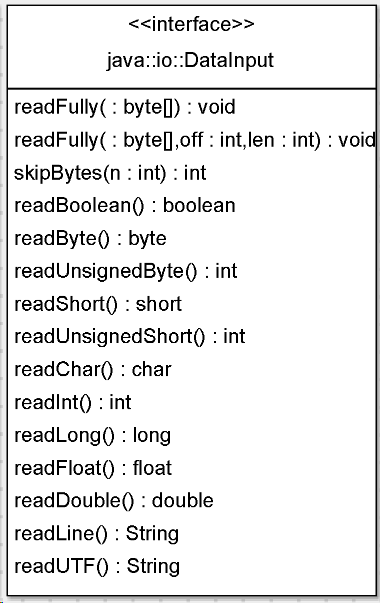
\includegraphics[width=1\linewidth]{UML/inputstream/datainput}
\caption{DataInput 接口的 UML 类图}
\label{fig:datainput}
\end{figure}

下面是这个接口的代码。
\begin{java}
interface DataInput {
\end{java}
首先显示两个读取全部字节的方法。
\begin{java}    
    void readFully(byte b[]) throws IOException;
    void readFully(byte b[], int off, int len) throws IOException;
\end{java}
然后是一个用于跳过一定字节数目的方法,或者说是读取不返回。
\begin{java}    
    int skipBytes(int n) throws IOException;
\end{java}
之后是一些用于从中读取Java基础类型的方法,从二进制流经行序列化。
\begin{java}   
    boolean readBoolean() throws IOException;
    byte readByte() throws IOException;
    int readUnsignedByte() throws IOException;
    short readShort() throws IOException;
    int readUnsignedShort() throws IOException;
    char readChar() throws IOException;
    int readInt() throws IOException;
    long readLong() throws IOException;
    float readFloat() throws IOException;
    double readDouble() throws IOException;
\end{java}
最后是读取一整行或者是读取 UTF 编码内容的内容。
\begin{java}
    String readLine() throws IOException;
    String readUTF() throws IOException;
}
\end{java}
